%Started on Monday 28 August 2006
%Aug: 29, 30
%Sep:  7,  8, 13
% 2007
%Feb:  4

%
% Chapter: Warm-start
%
\label{ch:Warmstart}

Stochastic programming \cite{BirgeLouveaux,KallWallace}
is a technique to inform decision-making 
in many areas of applied mathematics, engineering, economics and 
finance where some parameters are unknown.
%
Stochastic programming models uncertainty through the analysis 
of possible future outcomes (scenarios). We hope that the more detailed the 
description is, the more robust are the decisions taken. 

Taking into account a large number of possible scenarios leads
to the generation of large-scale structured optimization problems.
With the growing industrial acknowledgement of the benefits of 
considering uncertainty for planning purposes, it is expected that the 
need for solving very large instances will grow as well.
As the dimensions of the problems increase, the computational advantages 
of relying on interior point solvers become more and more evident. 

In this chapter we develop an efficient way of constructing a 
starting point for structured large-scale stochastic linear programs.

This chapter is designed as follows. We first present the relevant
concepts of stochastic programming and introduce a measure of
the distance between scenarios. Then we review some studies on 
warm-start techniques for interior point methods. Then we introduce 
the proposed method of generating a good starting point for 
stochastic programming that exploits the inherent structure of the
problem. Finally, we present an analysis of the warm-start strategy.

The results presented in this chapter have been the subject
of a joint work with Jacek Gondzio and Andreas Grothey
\cite{ColomboGondzioGrothey06}. 

%
% Section
%
\section{Stochastic programming}

By stochastic programming, we mean decision and control models in which 
data evolves over time, and are subject to significant uncertainty.
%
Uncertainty in the data is a commonly observed phenomenon in
optimization problems coming from applications. Uncertainty
affects problems that aim to plan future actions based on forecasted
prices or costs. In can be argued that nearly all practical
optimization problems display uncertainty in the data, even if this is
not made explicit in the chosen solution method. 

A crude approach to the problem of optimization under uncertainty
has been to replace the uncertain data by their expected value and
solve an {\em average case} problem. However, this approach is not
suitable when some sort of provision of hedging against risk has to be
taken into account. Another popular approach is {\em Robust
optimization}, or the optimization of the {\em worst case}
scenario \cite{KallWallace}. 

When the uncertainty cannot be conveniently forecasted, the use of 
deterministic models is considered inadequate for decision making. In 
these situations, being able to describe and model the uncertain parameters
becomes a requirement for robust decision making. Stochastic 
programming \cite{BirgeLouveaux,KallWallace} is the discipline that 
studies the methods and provides the tools for modelling uncertainty.

Stochastic programming aims to take all possible future scenarios 
into account, weighting them
with their respective probabilities. Its strength lies in the
adaptability which allows to express preferences such as restricting
the exposure to risk. Unlike alternative approaches, it allows to model
situations in which possible future events are correlated or follow a
time-structure, in that realisations become known in stages and it is
possible to react to the observed events.

\fb{
The stages do not necessarily refer to time periods, they correspond
to steps in the decision process. The main interest lies in the 
first-stage decisions which consist of all decisions that have to
be made before the information is revealed. Later-stage decisions 
are allowed to adapt to the information gathered up to that point.
}

Its perceived weaknesses are the need for reliable forecasts
of the probabilities of the future events under consideration
(which may not be available), and the fact that stochastic programming
(especially when applied to multi-stage models) tends to lead to
problems with very large dimensions, thus making their solution
challenging. 

%
%
\subsection{Stochastic programming concepts}

A stochastic programming problem incorporates the uncertain parameters
in the model, as can be illustrated by the problem
%
\be \label{eq:SP}
\min_x \E_\xi(f(x, \xi)) \;\text{ subject to }\; g(x, \xi) \le 0,
\ee
%
where $\xi$ is a random variable and $\E_\xi$ is the expectation function.
This can be interpreted as an optimization
problem in which some parameters or coefficients are unknown.
Formulation (\ref{eq:SP}) is however an unsatisfactory model, since
it is unclear how to interpret the {\em probabilistic} constraint
$g(x,\xi) \le 0$. A better formulation is the stochastic program
with recourse:
%
\begin{eqnarray} \label{eq:SPRecourse}
\min_x \hspace{-1.5em} && \E_\xi[f(x, \xi) + Q(x, \xi)] \nonumber \\ 
  && Q(x,\xi) = \min_y \{\, q(y) : u_i(y) \ge g_i^+(x, \xi),\:\forall i \,\},\\
  && g_i^+(x, \xi) = \max \{\, g_i(x, \xi), \, 0 \,\}. \nonumber
\end{eqnarray}

\fb{
Explain what the recourse is.
}

In stochastic programming, the uncertain environment is 
described through a stochastic process which is assumed to be 
known or can be either estimated from historical data or 
conjectured according to some prescribed properties. The 
continuous process $\xi$ is usually further approximated by a discrete 
distribution, $\xi \in \{\xi_1, \ldots,\xi_n\}$, $p(\xi=\xi_i) = p_i$,
in order to obtain a computationally amenable description. 
%
In such a case, the most common technique generates a 
finite, but usually very large, number of scenarios that represent an 
approximate description of the possible outcomes.

%The decision variables $x$ are
%split depending on the timing of the decision: $x_0$ are those
%variables whose value is to be decided {\em before} the random event
%becomes known, $x_i$ are decisions taken as a reaction to the outcome
%of $\xi$ being $\xi_i$ (recourse action). Problem
%(\ref{continuousSP}) then becomes
%\begin{equation}
%\min_{x} \sum_{i=1}^n p_i f(x_0, x_i, \xi_i)) \text{~subject
%to~}c(x_0, x_i, \xi_i) \le 0,
%\label{SP}
%\end{equation}

The model can be generalised to a multi-stage model in which 
the evolution of uncertainties can be 
described as an alternating sequence of decisions and random 
realisations that occur at different points in time (stages).
The discrete stochastic process can be represented as an event tree,
where each node denotes a stage when a realisation 
of the random process becomes known and a subsequent decision is taken.
A path from the root to a leaf node of the event tree represents a 
scenario.
A very simple event tree is shown in Figure~\ref{fig:EventTree}.
%
\begin{figure}[ht]
  \begin{center}
    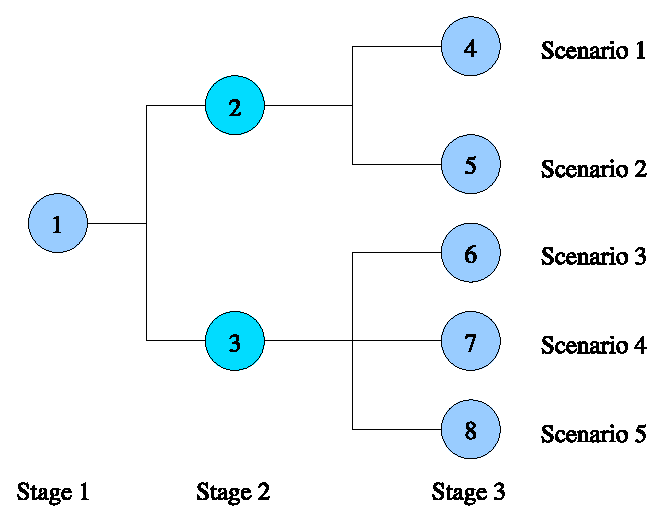
\includegraphics[scale=0.6]{figures/tree.eps}
    \caption{Event tree.}
    \label{fig:EventTree}
  \end{center}
  \vspace{-3ex}
\end{figure}

To each node of the event tree we associate a set of constraints, an 
objective function, and the conditional probability of visiting the 
node from its parent node in the previous stage.
The probability of each scenario is the product of the 
conditional probabilities of visiting each node on the path.

The question of how to generate an appropriate scenario tree
is not trivial, and has received extensive attention in the
literature 
\cite{DupacovaConsigliWallace,HoylandKautWallace,HoylandWallace,Pflug01}.

\fb{
It should be noted that usually a very large number of scenarios is
needed to adequately capture the characteristics of the underlying
continuous distribution, particularly in the multi-stage setting.
In this case, the number of scenarios grows exponentially with the
number of decisions considered at each stage.

The size of the scenario tree determines the size of the optimization
program.
}

%
%
\subsection{Deterministic equivalent formulation for stochastic programs}
\label{DetEqForm}

A natural formulation of a stochastic programming problem relies on 
recursion to describe the dynamics of the modelled process.
The term {\it recourse} means that, at each stage, the decision 
variables adapt to the different outcomes of the random parameters.

A multistage stochastic program with recourse is a multi-period 
mathematical program where parameters are assumed to be uncertain 
along the time path.

For ease of presentation, we consider the linear version of the
general recourse problem (\ref{eq:SPRecourse}):
%
\be \label{eq:SLPRecourse}
\begin{array}{rl}
\min & c^T x + \E_\xi[\min q(y)^T y(\xi)] \\
\raisebox{2.8ex}{\mbox{s.t.}} & \!\!\begin{array}{lcl}
	       Ax                       &=& b,     \\
	       T(\xi) x + W(\xi) y(\xi) &=& h(\xi), \\
	       x \geq 0,\; y(\xi) \ge 0,
	      \end{array}
\end{array}
\ee
%
where $y(\xi)$ denotes the recourse action which depends on the 
outcome of the random process $\xi$. After discretizing $\xi$ 
according to $P(x_i=\xi_i) = p_i$, and using the notation 
$T_i = T(\xi_i)$ (and analogously for $h_i$, $W_i$, $y_i$ and $q_i$), 
problem (\ref{eq:SLPRecourse}) can be written in the 
{\em deterministic equivalent formulation}:
\be \label{eq:DetEq-2stage}
\begin{array}{rlllll}
\min & c^T x + \sum_i p_iq_i^T y_i \\
\mbox{s.t.} & Ax              &        &          & = b,   \\
            & T_1 x + W_1 y_1 &        &          & = h_1  \\
	    & \vdots          & \hspace{-1em}\ddots & & \;\vdots \\
            & T_n x           &        &+\; W_n y_n & = h_n \\
            & x \geq 0,\; y_i \ge 0.
\end{array}
\ee

Problem (\ref{eq:DetEq-2stage}) displays dual-block angular structure
in the constraint matrix.

\fb{
Explain why deterministic.
}

To formulate the deterministic equivalent of the multi-stage 
stochastic programming problem we first need to enumerate all nodes 
of the event tree. We use a breadth-first 
search order, i.e., we start from a root node corresponding 
to the initial stage and end with leaf nodes corresponding 
to the last stage. In this case, the constrint matrix displays
a nested dual-block angular structure.

Let $t = 1,2,\ldots,T$ denote the stage and $l_t$ be the index of a 
node at stage $t$.
Let $L_t$ denote the last node at stage $t$. Hence 
the nodes that belong to stage $t > 1$ have indices 
$l_t = L_{t-1} \! + \! 1, L_{t-1} \! + \! 2, \dots, L_t$. 
With $a(l_t)$ we denote the direct ancestor of node $l_t$ (which is a 
node that belongs to stage $t-1$).

\fb{
For any node in the tree at stage $t$ there is only one immediate
ancestor at stage $t-1$ and a finite number of descendants at $t+1$.
}

All decision variables $x$ are superscripted with the node number 
$l_t$.

The main constraint that describes the dynamics of the system has the form 
\[
  T^{l_t}x^{a(l_t)} +W^{l_t}x^{l_t} =h^{l_t}, \qquad l_t =L_{t-1}+1,\dots,L_t,
\]
%
where $T^{l_t}$ is the technology matrix that varies 
with the node in the event tree, and $W^{l_t}$ is the recourse
matrix that, in general, depends on realisations within the same stage,
but often varies only with time.

The deterministic equivalent formulation of the multi-stage 
problem has the following general form:

\begin{equation}
  \begin{array}{rrclll}
    \min & (q^{l_1})^T x^{l_1} & + & \!\!\!\!{\displaystyle \sum_{l_2=L_1 \!+\! 1}^{L_2}} \!\!\! p^{l_2} (q^{l_2})^T x^{l_2} && \!\!\!\!\!\!  + \; \ldots \; + {\displaystyle \sum_{l_T = L_{T-1} \! + \! 1}^{L_T}} \!\!\!\!\! p^{l_T} (q^{l_T})^T x^{l_T} \\
    \mbox{s.t.} & & & W^{l_1} x^{l_1} & \hspace{-1.5cm} = h^{l_1}, \\
    & T^{l_2} x^1 & + & W^{l_2} x^{l_2} & \hspace{-1.5cm} = h^{l_2}, & l_2 = L_1 \!+\! 1,\dots,L_2, \\
    & & \vdots & & \hspace{-1.4cm} \vdots \\
    & T^{l_T} x^{a(l_T)} & + &  W^{l_T} x^{l_T} & \hspace{-1.5cm} = h^{l_T}, & l_T = L_{T-1} \! + \! 1, \dots, L_T, \\
    & & & x^{l_t} & \hspace{-1.5cm} \geq 0, & l_t = 1,\dots, L_{T}. \\
    \label{DetEquiv}
  \end{array} 
\end{equation}

Note that the probabilities in the objective function of problem 
(\ref{DetEquiv}) are the unconditional path probabilities: $p^n$ is 
the probability that a path goes through node $n$, which equals the 
product of the conditional probabilities along the path from the root 
to the node.

If the event tree is traversed with depth-first-search ordering of the 
nodes during the generation of the mathematical program, the 
corresponding constraint matrix displays a nested dual block-angular 
structure.
%
While the different ordering of blocks whithin the matrix is not 
relevant for general-purpose solvers, the
structure-exploiting software OOPS \cite{GondzioSarkissian} can take 
fully advantage of the nested structure.

\fb{
Kall and Mayer \cite{KallMayer} provided a comparison of different
solution algorithms for stochastic linear programming problems.
}

%
% Section
%
\section{Warm-start with interior point methods}
\label{sec:WarmStart}

Consider again the linear programming problem in standard form
\[
\min\;  c^T x \;\quad \mbox{s.t. }\; Ax = b, \;\; x \ge 0,
\]
where $A \in \R^{m \times n}$ is full rank, 
$x, c \in \R^{n}$ and $b \in \R^{m}$. 
As discussed in Section~\ref{sec:StartingPoint}, the problem of 
finding a starting point is usually solved by using 
Mehrotra's starting point heuristic \cite{Mehrotra92}, which is 
considered to be computationally effective for generic problems.

However, many practical applications rely on solving a sequence 
of closely related problems, where the instances differ by some 
perturbation. This happens within algorithms that are sequential 
in their nature, such as sequential linear programming or
sequential quadratic programming.
It is also very common in (mixed) integer programming, when the
problems are solved by relaxing the integrality constraints and
introducing some branching strategy, such as in branch-and-bound,
branch-and-cut, branch-and-price.
Similarly, sequential problems appear in the context of solution 
methods based on cutting planes.

In these situations, we expect the solution of an instance to be 
close to the solution of the next one, in the sense that some of
the information gathered in the solution process may still be valid. 
Therefore, (warm) starting the 
optimization of one problem from the solution of the previous one
should reduce the computational effort of solving the perturbed instance.

Warm-start techniques are very successful 
when implemented with a simplex solver (see, for example, 
\cite{Bixby02}). 

\fb{
More on the simplex.
}

However, in the context of interior point methods, it 
is much more difficult to implement successfully, for the reasons
we outline below.

%
%
\subsection{Difficulties}
\label{sec:WarmStartDifficulties}

An optimal solution of a linear programming problem found with 
interior point methods is very close to the optimal vertex of 
the feasible polytope. With changes in the polytope (e.g. because 
of the addition of cutting planes or other changes in the 
problem data), the optimal solution changes as well.
In such a case the previous solution is very close to a non optimal
vertex or, in other words, very far from the central path. 

The effectiveness of an interior point algorithm degrades when an 
iterate gets too close to a boundary before optimality is reached,
and when the iterate gets far from the central path.

\fb{
As said in Chapter~\ref{ch:Ipm}, interior point methods approach 
the solution to the KKT system of optimality conditions by relaxing 
the complementarity requirements.
This is equivalent to postponing the choice of the optimal partitioning.

Therefore, moving toward a vertex can be interpreted as making 
a decision on the optimal partitioning. If the vertex is not an 
optimal one, then the central path will not approach it.

Therefore the algorithm may spend many iterations in recovering
centrality, during which small steps are usually generated and thus
very slow progress is achieved.
}

Hipolito \cite{Hipolito} considered the issue of robustness of 
search directions in interior point methods in these situations.
In his analysis, Hipolito showed that if the iterate is close 
to a boundary, the affine-scaling direction may be parallel to 
the nearby constraints. In such cases, the corrector direction 
may also display the same behaviour, and short stepsizes are 
obtained for the resulting search direction.

The required features for a good warm-start candidate for an
interior point algorithm are somewhat contradictory.
The point should not be too close to the boundary of the feasible 
region in order to be able to absorb larger perturbations in the 
problem data. 
However, it should be sufficiently advanced to provide 
computational savings over a cold-start iterate.
A common way of accommodating these requirements is to store an 
approximate $\mu$-center well before reaching optimality 
\cite{Gondzio98,GondzioGrothey03,GondzioVial,YildirimWright}.

The theory and practice of warm-start techniques for interior point 
methods is a relatively new and still open field of study.
In the remainder of this section we present a review of some 
of the warm-start approaches proposed in the interior point literature.

%
%
\subsection{Changes in the problem size}

Mitchell \cite{Mitchell88} and Mitchell and Todd \cite{MitchellTodd}
analyse the potential reduction interior point method within
a cutting plane algorithm. They exploit the fact that
the primal feasible point can be constructed after a set of new
columns is added to the problem. They use this strategy with success
in column generation scheme and more generally in the solution 
of combinatorial optimization problems.

Gondzio \cite{Gondzio98} presents a warm-start procedure for 
primal--dual interior point methods in the context of a cutting 
plane method. The interior 
point method is used to solve a sequence of restricted master 
problems, which differ by one or more cutting planes.
%
% Therefore, by construction the solution to one problem violates 
% some of the newly added constraints.
% The optimal solution to a problem is necessarily very close 
% to the boundary, thus is an unattractive starting point 
% for a perturbed problem. Therefore, an alternative warm-start 
% iterate needs to be defined.
%
The idea proposed in \cite{Gondzio98} is to store a nearly optimal 
point (3--4 digits of accuracy) to be employed as a warm-start point.
%
% Because of the cutting plane setting, the problem is then solved 
% to optimality (7--8 digits of accuracy) in order to generate 
% appropriate cuts.
%
As one requirement for a good iterate is centrality, it is of interest 
to perform a few centering steps on the stored iterate, the cost of 
which is marginal, as a factorisation is already available. The 
recentering steps proposed are based on
centrality correctors \cite{Gondzio96}.
An auxiliary feasibility recovery procedure may be needed as, due to 
the addition of cuts, large infeasibilities are often produced.

% The role of interior point methods in integer and combinatorial 
% optimization has been comprehensively surveyed in \cite{Mitchell96} 
% and \cite{MitchellPardalosResende98}.

%
%
\subsection{Perturbations that do not affect the problem size}

Hipolito \cite{Hipolito} studies an alternative centering direction 
in the context of the dual affine-scaling algorithm. Such a 
direction is designed to move the iterate away from the boundary, 
overcoming the risk of moving parallel to it that was mentioned 
in Section~\ref{sec:WarmStartDifficulties}. 
By considering a weighted least squares formulation, Hipolito 
develops the dual affine-scaling and the corresponding Newton 
centering directions. 
This study has an immediate interest for warm-starting approaches,
as the resulting direction points towards the interior of the 
feasible region, thus providing the algorithm with the necessary 
space to make fast progress. 
Unfortunately, it is developed only for the dual affine-scaling 
algorithm, and to the best of our knowledge there have been no 
studies on how to obtain a similar search direction in the 
primal--dual context.

The warm-start approach proposed in \cite{Gondzio98} is extended
in \cite{GondzioVial} to the case of solving a sequence of problems 
with the same dimensions but changing problem data (the objective 
function or the right-hand side). Such situations arise 
in the context of decomposition approaches for large structured 
linear programs. 
In the case of Dantzig--Wolfe decomposition, successive subproblems 
differ only in the objective function, while in the case 
of Benders decomposition they differ only in the right-hand sides.
Following \cite{Gondzio98}, nearly optimal points are saved and used 
to warm start the solution of subsequent subproblems \cite{GondzioVial}.

% An advanced application of this technique is studied in 
% \cite{GondzioVial}, where a decomposition approach for large 
% structured linear programs is implemented within an interior point 
% framework. In this setting, a sequence of linear problems is generated 
% by adding cutting planes to provide a polyhedral approximation of a 
% non-differentiable convex function, and a warm-start strategy is 
% applied when solving each subproblem.

\yildirim and Wright \cite{YildirimWright} consider again the case 
of solving a sequence of problems in fixed dimensions, and
analyse the number of iterations required to converge to a 
solution of the perturbed instance from the warm-start point and 
obtain worst-case estimates.
They show that these estimates depend on the size of the perturbation 
as well as on the conditioning %and other properties 
of the problem 
instances. Thus they obtain conditions under which the complexity 
of the warm-start approach is better than for the cold start case.

The strategy proposed in \cite{YildirimWright} aims at correcting the 
primal and dual infeasibilities introduced by the perturbation in just 
one step.
% relying on the centrality of the iterate from one instance
% to provide enough centrality for the starting point of the next instance.
In this strategy, they backtrack to an iterate for which $\mu$ is 
large enough to allow a full step for the correction they produce. 
Hence, the amount of necessary backtracking depends on the magnitude 
of the perturbation.
This is intuitively justified considering that a large perturbation 
will produce a large adjustment, and it is essential to guarantee that 
a full step will not compromise the non-negativity requirements of the 
iterate.
%
To ensure the availability of an approximate $\mu$-center from which 
the perturbation can be absorbed in one step, a subset of 
iterates for different values of $\mu$ is stored.
When the size of the perturbation becomes known, the closest $\mu$ 
available is retrieved, and the corresponding iterate is used as a 
warm-start point for the next problem in the sequence.
%
In \cite{YildirimWright}, two different corrections for the perturbation
are studied: one is based on least squares, the other on a Newton step 
correction.
A detailed computational comparison of these strategies has been 
carried out by John and \yildirim \cite{JohnYildirim}.

Gondzio and Grothey \cite{GondzioGrothey03} propose a different 
reoptimization technique for interior point methods.
As in \cite{YildirimWright}, they aim at obtaining conditions for 
perturbations that can be absorbed in one Newton step.
Hence, they introduce a relative measure of perturbations, in which 
the primal and the dual spaces are analysed independently.

%They derive the directions for absorbing primal and dual 
%infeasibilities from the system
%\[
%\left[ \begin{array}{ccc}
%    A & 0 & 0 \\ 0 &A^T & I \\ S & 0 & X
%  \end{array} \right]
%\left[ \begin{array}{c}
%    \Delta x \\ \Delta \lambda \\ \Delta s
%  \end{array} \right] = 
%\left[ \begin{array}{c}
%    -r_b \\ -r_c \\ 0
%  \end{array} \right].
%\]
%This formulation aims at restoring feasibility, while the requirement 
%for a well-centred iterate is considered separately. 

Their reoptimization procedure is based on two phases: first, an attempt 
is made to absorb the infeasibilities caused by the perturbation with a full 
Newton step; second, the centrality of the iterate is improved.
Another key feature of their approach is that the primal search 
direction is governed only by the primal perturbation, and similarly 
for the dual space. This corresponds to solving the Newton system 
(\ref{eq:NewtonSystem}) for the two right-hand sides independently
%
\be \label{eq:NewtonSystem2}
\left[ \begin{array}{ccc}
    A & 0 & 0 \\ 0 &A^T & I \\ S & 0 & X
  \end{array} \right]
\left[ \begin{array}{c}
    \Delta x \\ \Delta y \\ \Delta s
  \end{array} \right] = 
\left[ \begin{array}{c}
    \xi_b \\ 0 \\ 0
  \end{array} \right] +
\left[ \begin{array}{c}
    0 \\ \xi_c \\ 0
  \end{array} \right].
\ee
%
They produce bounds on the magnitude of primal perturbation $\xi_b$ 
and dual perturbation $\xi_c$ that can be absorbed in a single 
Newton step. As opposed to the results of \cite{YildirimWright}, 
the bounds of \cite{GondzioGrothey03} are easy to compute and 
thus can be used in practice.

If the perturbation is bounded above by some quantity depending 
on $n$ and $\theta$, a full Newton step can be taken in the dual space. 
This happens for both the $\mathcal{N}_2$ and $\mathcal{N}_\infty$ 
neighbourhoods. Similarly, a full Newton step can be taken in the 
primal feasibility restoration direction. These conditions may not 
be satisfied in practice. In such case, a different iterate further 
away from optimality may be more likely to allow for a full Newton step.

A practical implementation is developed within an infeasible interior 
point method. In this context, a stronger emphasis may be put on 
reducing the infeasibilities. This is accomplished with additional 
centering steps.

An approximate $\mu$-center is stored for a tolerance level that 
depends on the magnitude of the expected perturbation. This does not 
exclude the possibility of storing a sequence of iterates, as proposed 
in \cite{YildirimWright}, thus postponing the choice of the one to 
use.
As the problem size does not change, an approximate $\mu$-center 
can immediately be used as an iterate for the next problem.
If only one iterate is stored, then the absorption of infeasibilities 
may be spread across a few iterations whenever the stepsizes fall 
below a predefined level.

As this strategy does not make assumptions upon the centrality of the 
warm-start iterate,
% (as opposed to what is assumed in \cite{YildirimWright}), 
it can be initialised with any iterate.
Gondzio and Grothey \cite{GondzioGrothey03} apply this warm-start 
strategy successfully to structured problems for crash-start points that 
come from a cross-decomposition scheme, and thus may lack centrality.

% This feature is exploited when we use a warm-start iterate generated
% from a reduced event tree, as discussed in the following sections.

A different approach has been studied by Benson and Shanno 
\cite{BensonShanno}. They investigate how to improve the efficiency 
of interior point methods in a reoptimization context by the use of 
a primal--dual penalty approach.
While standard penalty techniques are effective only in one space, 
the introduction of penalty parameters in both the primal and the 
dual problems allows to capture perturbations in both spaces.
%
% For example, an $l_1$ penalty can deal with changes in the right-hand
% side of the constraints (primal changes), but has virtually no effect
% in perturbations of the objective coefficients (dual changes).
%
The penalised problem allows the variables to become negative, with
the immediate advantage of accepting larger stepsizes along 
the computed search direction, thus favouring a faster progress
especially in the first few iterations.
% This is of particular importance in reoptimization, as the optimal
% solution of the previous problem is necessarily close to a boundary.


\hrulefill


Large or huge-scale problems, however, create more than one difficulty 
to general purpose solvers. Problems of these sizes can be solved by 
exploiting the structure present in the matrix. A further advantage 
comes from assigning the work to be done to more than one processing unit. 
This is where structure-exploiting parallel solvers such as OOPS 
\cite{GondzioSarkissian} excel. Moreover, structure-exploiting interior 
point methods can be used not only for linear programming problems, 
but also for quadratic and nonlinear problems \cite{GondzioGrothey04}.

In a large scenario tree there may be very little difference among 
scenarios, and so the large-scale problem can provide a fine-grained 
solution to a problem that could have been solved more coarsely by 
using a much smaller tree. This observation suggests a
warm-start technique that can be applied in the context of interior 
point methods. A warm-start solution is obtained by solving the 
stochastic optimization problem for a reduced event tree, whose 
dimension is much smaller than that of the complete one. The solution 
to the reduced problem is used to construct an advanced iterate for 
the complete formulation. We provide evidence that this novel way 
of exploiting the problem structure to generate an initial point 
provides a better iterate (in terms of centrality, feasibility, 
and closeness to optimality) than the one produced by a generic 
strategy.


%
%%%%%%%%%%%%%%%%%%%%%%%%%%%%%%%%%%%%%%%%%%%%%%%%%%%%%%%%%%%%%%%%%%%%%%%%%
%


%
% Section
%

%
% Section
%
\section{Other stuff}

\begin{itemize}
\item The reduced tree approach to construct a warmstart iterate 
doesn't seem to be IPM specific, and could be exploited also by a 
simplex solver (in which case, how would such a solver obtain the 
complete basis?). However, the advantage of IPM are the possibility 
of solving huge scale problems, parallelism, and extension to 
quadratic problems.

\item Provide a comparison between initial infeasibilities 
produced by Mehrotra's heuristic and the reduced-tree starting 
point. It would be great to have some sort of theoretical back-up 
about the relationship between magnitude of perturbation and 
initial infeasibilities.

\item Point out that the way we generate our starting point 
guarantees better centrality (at least in the sense of 
complementary pairs). Possibly this could be compared again 
with the points generated by Mehrotra's starting point heuristic.

\item Explain what we do with probabilities: how we adjust them 
in the reduced tree, and how they affect the dual iterates.

\item Point out that if we knew about the underlying 
stochastic process, then we could exploit it directly in the 
generation of the reduced tree (althogh, in such a case how 
could we ensure the correspondence of nodes between the reduced 
and the complete tree?)

\item Compare the efficiency of the strategy according to the 
number of variations in the stochastic file. Also, how many 
variations happen in our test problems?

\item Clarify the issue of nonanticipativity constraints: 
since we have our own deterministic equivalent generator, we 
already avoid duplication without using those constraints.

\fb{
Nonanticipativity means that the decisions taken at any stage 
do not depend on future realizations of the random parameter or 
on future decisions, but only on the history.
}

\item Mention that if the iterate produced by a reduced tree 
is not good enough (according to what criteria?), another one 
can be produced by generating a modified reduced tree (more 
bushy for example).
\end{itemize}


\subsection{Theoretical analysis}

Once we formulate the complete deterministic equivalent $A$, we need 
to satisfy the following system:
\[
Ax=b,
\]
where $A\in \R^{m\times n}$ is a block-structured matrix of 
large dimension. Since this is a challenging task, we consider 
only a fraction of the scenarios we are interested in. Therefore, 
instead of the complete event tree, we will focus on a subtree. 
This corresponds to partitioning the deterministic equivalent 
like this:
\[
A = \left[ \begin{array}{cc}
    \tilde{A} & 0 \\ Q & T \\
    \end{array} \right],
\]
where $\tilde{A}$ contains only the scenarios corresponding 
to the subtree, $T$ contains the remaining scenarios, and $Q$ 
provides the linking blocks. For computational purposes, the 
dimension of $\tilde{A}$ is much smaller than that of $A$.

Therefore, to obtain a warm-starting solution we need to solve 
the reduced system
\[
\tilde{A}\tilde{x}=\tilde{b},
\]
where we adopted a similar partitioning for $x$ and $b$.

In the context of primal--dual interior point methods, we are 
solving the system
\[
\left[ \begin{array}{ccc}
    \tilde{A} & 0 & 0 \\
    0 & \tilde{A}^T & I \\
    \tilde{S} & 0 & \tilde{X}
    \end{array} \right]
\left[ \begin{array}{c}
    \Delta\tilde{x} \\ \Delta\tilde{y} \\ \Delta\tilde{s}
\end{array} \right] = 
\left[ \begin{array}{c}
      0 \\ 0 \\ -\tilde{X}\tilde{S}e - \sigma\mu e
\end{array} \right]
\]

Given an optimality tolerance $\epsilon$, we need to solve 
the above system for some primal--dual solution 
$(\tilde{x}^*, \tilde{s}^*, \tilde{y}^*)$. This will be used 
as a warm-starting iterate for the complete system.

We face now the problem of how to reconcile the solution from 
the subtree to the solution for the complete tree.

\hrulefill

Later stages are the more subject to variation because they 
depend on the realisations of all previous stages. Stages 
closer to the root display less variability when additional 
scenarios are considered.

%
%
\subsection{Initialising the warm-start iterate}

As observed in the literature review above, the perturbations 
studied were of two types:
\begin{itemize}
\item changes in the data that do not affect the problem size;
\item changes that affect the problem size, by increasing the 
number of constraints (in either the primal or the dual problem).
\end{itemize}

In our approach, we have to face a different sort of 
perturbation, where the size of the problem changes in both 
the number of constraints and the number of variables in the 
primal and in the dual. Therefore, we are faced with the 
challenge of using the solution of the small instance to 
provide a warm-start iterate for the complete system. This 
entails initialising both the primal and the dual vectors, of 
which only a fraction of the elements are known. This objective 
can be achieved by exploiting the inherent structure of the problem.

We start by showing how to initialise the warm-start iterate 
in the simplest case possible. Let the primal problem be
\[
\begin{array}{rllllll}
  \min & c^T x_0 &+ c_1^Tx_1 &+ c_2^Tx_2 &+ c_3^Tx_3 \\
  \mbox{s.t.} & Fx_0 &   \!\!\! + \; Gx_1 &&& = & b_1 \\
              & Fx_0 &&  \!\!\! + \; Gx_2 &&  = & b_2 \\
              & Fx_0 &&& \!\!\! + \; Gx_3 &   = & b_3 \\
              & x_i &\ge 0, &i = 0, 1, 2, 3.
\end{array}
\]

Note that the technology matrix $F$ and the recourse matrix 
$G$ are the same for all scenarios. This fact is fundamental 
in our approach, and is not overly simplistic: many real life 
situations are modelled this way. 

Suppose we solve a reduced problem with only two scenarios. 
While such a reduction is not sensible in practice, it will 
make our approach evident.

%
%
\subsection{Dual initialisation}

After having solved the reduced problem, we want to obtain 
proper initial values for $(x_3, y_3, s_3)$. To do this, let 
us consider the dual formulation (WHY?)
\[
\begin{array}{rrrrllllll}
\max & b_1^T y_1 & \!\!\! + \;\,\, b_2^T y_2 & \!\!\! + \;\,\, b_3^T y_3 \\
\mbox{s.t.} & F^T y_1 & \!\!\! + \; F^Ty_2 & \!\!\! +\; F^Ty_3 & \!\!\! +\; s_0 &&&& \!\!\!= c_0 \\
            & G^T y_1 &&&& \!\!\! + \; s_1 &&&  \!\!\!= c_1 \\
            && G^T y_2 &&&&  \!\!\! + \; s_2 && \!\!\!= c_2 \\
            &&& G^T y_3 &&&& \!\!\! + \; s_3 &  \!\!\!= c_3 \\
            &&&&&&&& \hspace{-7.8cm} s_i \ge 0, \quad i = 0, 1, 2, 3.
\end{array}
\]

We notice that the last set of equations depends only on the 
newly added variables. Hence, we may want to find a feasible 
solution with respect to these constraints. By neglecting the 
first set of constraints, we will likely violate them. We accept 
this as the unavoidable price to pay if we want to find a 
computationally viable starting point.

By linearity, if we find weights $\omega_1$ and $\omega_2$ such that
\[
  \omega_1 c_1 + \omega_2 c_2 = c_3,
\]
then we would immediately retrieve $y_3$ and $s_3$:
\[
  y_3 = \omega_1 y_1 + \omega_2 y_2, \quad s_3 = \omega_1 s_1 + \omega_2 s_2.
\]

However, without imposing conditions on $\omega_1$ and $\omega_2$, 
we have no guarantee to obtain $s_3 \ge 0$.

Let us first consider the unconstrained subproblem. As the system 
is overdetermined, we aim for a least squares solution. Hence we 
try to find weights such that
\[
  \min \; \| c_3 - C\omega\|_2^2,
\]
where $C = [c_1 \; c_2]$ and $\omega = [\omega_1 \; \omega_2]^T$. 
This corresponds to
\[
  \min \; (c_3 - C\omega)^T(c_3 - C\omega),
\]
whose solution satisfies
\[
  C^T C\omega = C^T c_3.
\]

Let us now turn to the constrained problem
\begin{eqnarray*}
  &\min &(c_3 - C\omega)^T(c_3 - C\omega) \\
  &\mbox{s.t.} &Sw \ge 0,
\end{eqnarray*}
where $S = [s_1 \; s_2]$. The solution to this problem satisfies
\[
  C^T C\omega = C^T c_3 + \frac{1}{2}S^T\lambda,
\]
where $\lambda$ is the vector of Lagrange multipliers and can be 
used to penalise solutions that violate the non-negativity 
constraints. We first set $\lambda = 0$ and thus solve the 
unconstrained problem. If this produces an iterate $s_3 \ge 0$, 
then we are done. Otherwise, we set $\lambda^{(j)} > 0$ for the 
components $s_3^{(j)} <0$ and solve again. This may need to be 
repeated until we obtain weights $\omega$ for which $S\omega \ge 0$.

This ad-hoc mechanism may be too complicated to be 
computationally viable. Another possibility is to solve the 
constrained problem as a quadratic programming problem. However, 
this possibility may still require more effort than what 
we are willing to use.

For a practical implementation, we may resort to the simpler 
strategy of shifting any negative values of $S\omega$. 
We observe that a similar approach is used in finding the starting 
point for interior point methods \cite{Mehrotra92}.

%
%
\subsection{Primal initialisation}

How to initialise the primal variables:
\begin{itemize}
\item From dual such that $x_3s_3 = \mu$;
\item From $Gx_3 = b_3 - Fx_0$ (maybe plus additional conditions 
on centrality since it's an underdetermined system).
\end{itemize}
